\documentclass[12pt,letterpaper,fleqn]{hmcpset}
\usepackage[margin=1in]{geometry}
\usepackage{graphicx}
\usepackage{amsmath,amssymb}
\usepackage{enumerate}
\usepackage{hyperref}
\usepackage{parskip}

% Theorems
\usepackage{amsthm}
\renewcommand\qedsymbol{$\blacksquare$}
\makeatletter
\@ifclassloaded{article}{
    \newtheorem{definition}{Definition}[section]
    \newtheorem{example}{Example}[section]
    \newtheorem{theorem}{Theorem}[section]
    \newtheorem{corollary}{Corollary}[theorem]
    \newtheorem{lemma}{Lemma}[theorem]
}{
}
\makeatother

% Random Stuff
\setlength\unitlength{1mm}

\newcommand{\insertfig}[3]{
\begin{figure}[htbp]\begin{center}\begin{picture}(120,90)
\put(0,-5){\includegraphics[width=12cm,height=9cm,clip=]{#1.eps}}\end{picture}\end{center}
\caption{#2}\label{#3}\end{figure}}

\newcommand{\insertxfig}[4]{
\begin{figure}[htbp]
\begin{center}
\leavevmode \centerline{\resizebox{#4\textwidth}{!}{\input
#1.pstex_t}}
\caption{#2} \label{#3}
\end{center}
\end{figure}}

\long\def\comment#1{}

\newcommand\norm[1]{\left\lVert#1\right\rVert}
\DeclareMathOperator*{\argmin}{arg\,min}
\DeclareMathOperator*{\argmax}{arg\,max}

% bb font symbols
\newfont{\bbb}{msbm10 scaled 700}
\newcommand{\CCC}{\mbox{\bbb C}}

\newfont{\bbf}{msbm10 scaled 1100}
\newcommand{\CC}{\mbox{\bbf C}}
\newcommand{\PP}{\mbox{\bbf P}}
\newcommand{\RR}{\mbox{\bbf R}}
\newcommand{\QQ}{\mbox{\bbf Q}}
\newcommand{\ZZ}{\mbox{\bbf Z}}
\renewcommand{\SS}{\mbox{\bbf S}}
\newcommand{\FF}{\mbox{\bbf F}}
\newcommand{\GG}{\mbox{\bbf G}}
\newcommand{\EE}{\mbox{\bbf E}}
\newcommand{\NN}{\mbox{\bbf N}}
\newcommand{\KK}{\mbox{\bbf K}}
\newcommand{\KL}{\mbox{\bbf KL}}

% Vectors
\renewcommand{\aa}{{\bf a}}
\newcommand{\bb}{{\bf b}}
\newcommand{\cc}{{\bf c}}
\newcommand{\dd}{{\bf d}}
\newcommand{\ee}{{\bf e}}
\newcommand{\ff}{{\bf f}}
\renewcommand{\gg}{{\bf g}}
\newcommand{\hh}{{\bf h}}
\newcommand{\ii}{{\bf i}}
\newcommand{\jj}{{\bf j}}
\newcommand{\kk}{{\bf k}}
\renewcommand{\ll}{{\bf l}}
\newcommand{\mm}{{\bf m}}
\newcommand{\nn}{{\bf n}}
\newcommand{\oo}{{\bf o}}
\newcommand{\pp}{{\bf p}}
\newcommand{\qq}{{\bf q}}
\newcommand{\rr}{{\bf r}}
\renewcommand{\ss}{{\bf s}}
\renewcommand{\tt}{{\bf t}}
\newcommand{\uu}{{\bf u}}
\newcommand{\ww}{{\bf w}}
\newcommand{\vv}{{\bf v}}
\newcommand{\xx}{{\bf x}}
\newcommand{\yy}{{\bf y}}
\newcommand{\zz}{{\bf z}}
\newcommand{\0}{{\bf 0}}
\newcommand{\1}{{\bf 1}}

% Matrices
\newcommand{\Ab}{{\bf A}}
\newcommand{\Bb}{{\bf B}}
\newcommand{\Cb}{{\bf C}}
\newcommand{\Db}{{\bf D}}
\newcommand{\Eb}{{\bf E}}
\newcommand{\Fb}{{\bf F}}
\newcommand{\Gb}{{\bf G}}
\newcommand{\Hb}{{\bf H}}
\newcommand{\Ib}{{\bf I}}
\newcommand{\Jb}{{\bf J}}
\newcommand{\Kb}{{\bf K}}
\newcommand{\Lb}{{\bf L}}
\newcommand{\Mb}{{\bf M}}
\newcommand{\Nb}{{\bf N}}
\newcommand{\Ob}{{\bf O}}
\newcommand{\Pb}{{\bf P}}
\newcommand{\Qb}{{\bf Q}}
\newcommand{\Rb}{{\bf R}}
\newcommand{\Sb}{{\bf S}}
\newcommand{\Tb}{{\bf T}}
\newcommand{\Ub}{{\bf U}}
\newcommand{\Wb}{{\bf W}}
\newcommand{\Vb}{{\bf V}}
\newcommand{\Xb}{{\bf X}}
\newcommand{\Yb}{{\bf Y}}
\newcommand{\Zb}{{\bf Z}}

% Calligraphic
\newcommand{\Ac}{{\cal A}}
\newcommand{\Bc}{{\cal B}}
\newcommand{\Cc}{{\cal C}}
\newcommand{\Dc}{{\cal D}}
\newcommand{\Ec}{{\cal E}}
\newcommand{\Fc}{{\cal F}}
\newcommand{\Gc}{{\cal G}}
\newcommand{\Hc}{{\cal H}}
\newcommand{\Ic}{{\cal I}}
\newcommand{\Jc}{{\cal J}}
\newcommand{\Kc}{{\cal K}}
\newcommand{\Lc}{{\cal L}}
\newcommand{\Mc}{{\cal M}}
\newcommand{\Nc}{{\cal N}}
\newcommand{\Oc}{{\cal O}}
\newcommand{\Pc}{{\cal P}}
\newcommand{\Qc}{{\cal Q}}
\newcommand{\Rc}{{\cal R}}
\newcommand{\Sc}{{\cal S}}
\newcommand{\Tc}{{\cal T}}
\newcommand{\Uc}{{\cal U}}
\newcommand{\Wc}{{\cal W}}
\newcommand{\Vc}{{\cal V}}
\newcommand{\Xc}{{\cal X}}
\newcommand{\Yc}{{\cal Y}}
\newcommand{\Zc}{{\cal Z}}

% Bold greek letters
\newcommand{\alphab}{\hbox{\boldmath$\alpha$}}
\newcommand{\betab}{\hbox{\boldmath$\beta$}}
\newcommand{\gammab}{\hbox{\boldmath$\gamma$}}
\newcommand{\deltab}{\hbox{\boldmath$\delta$}}
\newcommand{\etab}{\hbox{\boldmath$\eta$}}
\newcommand{\lambdab}{\hbox{\boldmath$\lambda$}}
\newcommand{\epsilonb}{\hbox{\boldmath$\epsilon$}}
\newcommand{\nub}{\hbox{\boldmath$\nu$}}
\newcommand{\mub}{\hbox{\boldmath$\mu$}}
\newcommand{\zetab}{\hbox{\boldmath$\zeta$}}
\newcommand{\phib}{\hbox{\boldmath$\phi$}}
\newcommand{\psib}{\hbox{\boldmath$\psi$}}
\newcommand{\thetab}{\hbox{\boldmath$\theta$}}
\newcommand{\taub}{\hbox{\boldmath$\tau$}}
\newcommand{\omegab}{\hbox{\boldmath$\omega$}}
\newcommand{\xib}{\hbox{\boldmath$\xi$}}
\newcommand{\sigmab}{\hbox{\boldmath$\sigma$}}
\newcommand{\pib}{\hbox{\boldmath$\pi$}}
\newcommand{\rhob}{\hbox{\boldmath$\rho$}}

\newcommand{\Gammab}{\hbox{\boldmath$\Gamma$}}
\newcommand{\Lambdab}{\hbox{\boldmath$\Lambda$}}
\newcommand{\Deltab}{\hbox{\boldmath$\Delta$}}
\newcommand{\Sigmab}{\hbox{\boldmath$\Sigma$}}
\newcommand{\Phib}{\hbox{\boldmath$\Phi$}}
\newcommand{\Pib}{\hbox{\boldmath$\Pi$}}
\newcommand{\Psib}{\hbox{\boldmath$\Psi$}}
\newcommand{\Thetab}{\hbox{\boldmath$\Theta$}}
\newcommand{\Omegab}{\hbox{\boldmath$\Omega$}}
\newcommand{\Xib}{\hbox{\boldmath$\Xi$}}

% mixed symbols
\newcommand{\sinc}{{\hbox{sinc}}}
\newcommand{\diag}{{\hbox{diag}}}
\renewcommand{\det}{{\hbox{det}}}
% \newcommand{\trace}{{\hbox{tr}}}
% \newcommand{\tr}{\trace}
\newcommand{\sign}{{\hbox{sign}}}
\renewcommand{\arg}{{\hbox{arg}}}
\newcommand{\var}{{\hbox{var}}}
\newcommand{\cov}{{\hbox{cov}}}
\renewcommand{\Re}{{\rm Re}}
\renewcommand{\Im}{{\rm Im}}
\newcommand{\eqdef}{\stackrel{\Delta}{=}}
\newcommand{\defines}{{\,\,\stackrel{\scriptscriptstyle \bigtriangleup}{=}\,\,}}
\newcommand{\<}{\left\langle}
\renewcommand{\>}{\right\rangle}
\newcommand{\Psf}{{\sf P}}
\newcommand{\T}{\top}
\newcommand{\m}[1]{\begin{bmatrix} #1 \end{bmatrix}}


\usepackage{physics}
\usepackage{fourier}

% info for header block in upper right hand corner
\name{Colin Adams}
\class{Math189R SU20}
\assignment{Homework 7}
\duedate{July 2020}

\begin{document}

Feel free to work with other students, but make sure you write up the homework
and code on your own (no copying homework \textit{or} code; no pair programming).
Feel free to ask students or instructors for help debugging code or whatever else,
though.
\newline
\newline
The starter files for problem 2 can be found under the Resource tab on course website. The plot for problem 2 generated by the sample solution has been included in the starter files for reference. Please print out all the graphs generated by your own code and submit them together with the written part, and make sure you upload the code to your Github repository.

\begin{problem}[1]
\textbf{(Murphy 11.3 - EM for Mixtures of Bernoullis)} Show that the M step for ML estimation
of a mixture of Bernoullis is given by
\[
    \mu_{kj} = \frac{\sum_i r_{ik}x_{ij}}{\sum_i r_{ik}}.
\]
Show that the M step for MAP estimation of a mixture of Bernoullis with a $\beta(a,b)$ prior
is given by
\[
    \mu_{kj} = \frac{\left(\sum_i r_{ik}x_{ij}\right) + a - 1}{\left(\sum_i r_{ik}\right) + a + b - 2}.
\]
\end{problem}
\begin{solution}
Okay, so we are maximizing a weighted sum of $ p(\vb x_i | \thetab_k)$ which is the same thing as maximizing its logarithm. To do that, we take the logarithm of it
\begin{align*}
\sum_{ij} r_{ij} \log p(\vb x_i | \thetab_j) = \sum_{ij} r_{ij} \sum_k \vb x_{ij} \log  \mub_{jk} + (1 - \vb x_{ij})\log(1 - \mub_{jk})
\end{align*}
which we take the gradient of with respect to $\mub_{jk}$ which gives us
\begin{align*}
\grad_{\mub_{jk}} \sum_{ij} r_{ij} \log p(\vb x_i | \thetab_j) = \sum_i r_{ij} \qty(\frac{\vb x_{ij} - \mub_{jk}}{\mub_{jk}(1 - \mub_{jk})}).
\end{align*}
Setting this to zero, we find that
\begin{align*}
\sum_i r_{ij} \vb x_{ij} = \sum_i r_{ij} \mub_{jk} \qquad \Rightarrow \mub_{jk} = \frac{1}{\sum_i r_{ij}}\sum_i r_{ij} \vb x_{ij}
\end{align*}
which we wished to show. 

Now if we do a similar thing, except we have a prior belief (i.e.\ the MAP maximization), we hope to maximize a mixture of $p(\vb x_i | \mub_k) p(\mub_k)$ where $p(\mub_k) \sim \beta(a,b)$. Again, this is the same thing as maximizing the log of that, so writing that out we have
\begin{align*}
\sum_{ij} r_{ij} \log p(\vb x_i | \mub_k) p(\mub_k) = \sum_{ij} r_{ij} \log p(\vb x_i | \mub_k)  + \log p(\mub_k).
\end{align*}
The first term is the same as above and the second term is very similar, so we have
\begin{align*}
\sum_{ij} r_{ij} \log p(\vb x_i | \mub_k)  + \log p(\mub_k) = \sum_{ij} r_{ij} \sum_k & \vb x_{ij} \log  \mub_{jk} + (1 - \vb x_{ij})\log(1 - \mub_{jk}) \\ &+ (a-1) \log  \mub_{jk} + (b - 1) \log (1 - \log \mub_{jk}). 
\end{align*}
Taking the derivative of this monstrosity with respect to $\mub$ gives us, after a few pages of algebra and some help from Mathematica, 
\begin{align*}
\grad_{\mub} ({\rm above}) = \frac{1}{\mub_{jk}(1 - \mub{jk})} \qty[\sum_i r_{ij} \vb x_{ij}  + (a - 1) - \mub_{jk}\qty((a -1) + (b -1) + \sum_i r_{ij})].
\end{align*}
Set [$\cdot$]'s to zero, and we can solve for $\mub_{jk}$ which gives us 
\begin{align*}
\mub_{jk} = \frac{\sum_i r_{ij} \vb x_{ij} + (a - 1)}{(a -1) + (b -1) + \sum_i r_{ij}}
\end{align*}
which is what we wished to show.



\vfill
\end{solution}
\newpage



\begin{problem}[2]
\textbf{(Lasso Feature Selection)} 
In this problem, we will use the online news popularity dataset we used in hw2pr3. In the starter code, we have already parsed the data for you. However, you might need internet connection to access the data and therefore successfully run the starter code.
\newline
\newline
First, ignoring undifferentiability at $x=0$, take $\frac{\partial |x|}{\partial x}
= \mathrm{sign} (x)$. Using this, show that $\nabla \|\xx\|_1 = \mathrm{sign}(\xx)$ where $\mathrm{sign}$ is applied
elementwise. Derive the gradient of the $\ell_1$ regularized linear regression objective
\begin{align*}
    \text{minimize: } & \|A\xx - \bb\|_2^2 + \lambda \|\xx\|_1
\end{align*}

Then, implement a gradient descent based solution of the above optimization problem for this data. Produce
the convergence plot (objective vs. iterations) for a non-trivial value of $\lambda$.
In the same figure (and different axes) produce a `regularization path' plot. Detailed
more in section 13.3.4 of Murphy, a regularization path is a plot of the optimal weight on
the $y$ axis at a given regularization strength $\lambda$ on the $x$ axis. Armed with this
plot, provide an ordered list of the top five features in predicting the log-shares of a news
article from this dataset (with justification).
\end{problem}
\begin{solution}
Doing the math bit, we have a given data vector $\vb x$, so 
\begin{align*}
\grad \norm{\vb x}_1 = \grad \sum_i \abs{x_i} = \sum_i \sign( x_i) \vu e = \sign(\vb x).
\end{align*}
Okay, if we hope to minimize $\norm{\vb A \vb x - \vb b}^2_2 + \lambda \norm{\vb x}_1$ then we just take the gradient and set to zero and all that so, using our matrix calculus rules we get
\begin{align*}
 0 = \grad(\norm{\vb A \vb x - \vb b}^2_2 + \lambda \norm{\vb x}_1) = \lambda \sign(\vb x) + 2(\vb A^T \vb A \vb x - \vb b^T \vb A) \qquad \Rightarrow \frac{\lambda}{2}\sign(\vb x) = \vb A^T \vb A \vb x - \vb b^T \vb A.
\end{align*}

 \begin{center}
     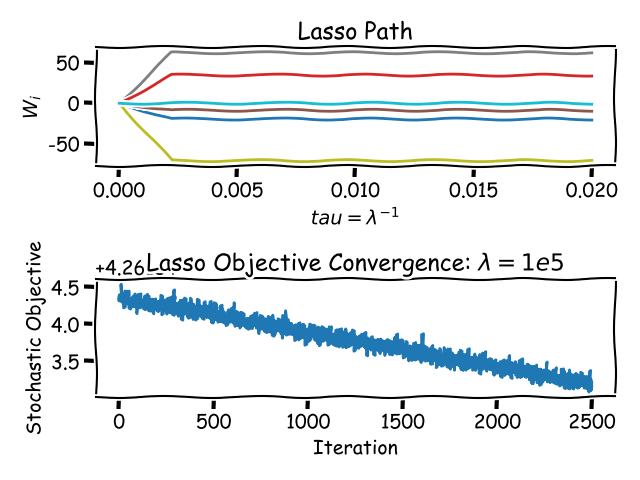
\includegraphics[width = 4.in]{hw7_starter_files/hw7pr2_lasso.png}
 \end{center}
Apparently the most important features are \texttt{[`timedelta', `weekday\_is\_wednesday', `weekday\_is\_thursday',
 `weekday\_is\_friday', `weekday\_is\_saturday']} and our plot is given above.



\end{solution}
\newpage

\end{document}
